%1. Intro White-box, overview of analysis
%2. Explaining some analyzing strats that are out there
%3. VaRA, explain what vara does roughly (Regions)
%4. Vara TS Experiment explain
%5  TEF Report and how we evaluate them
%6. Using data to build multiple perf-influcence models


\colorlet{punct}{red!60!black}
\definecolor{background}{HTML}{EEEEEE}
\definecolor{delim}{RGB}{20,105,176}
\colorlet{numb}{magenta!60!black}
\lstdefinelanguage{json}{
    basicstyle=\normalfont\ttfamily,
    numbers=left,
    numberstyle=\scriptsize,
    stepnumber=1,
    numbersep=8pt,
    showstringspaces=false,
    breaklines=true,
    frame=lines,
    backgroundcolor=\color{background},
    literate=
     *{0}{{{\color{numb}0}}}{1}
      {1}{{{\color{numb}1}}}{1}
      {2}{{{\color{numb}2}}}{1}
      {3}{{{\color{numb}3}}}{1}
      {4}{{{\color{numb}4}}}{1}
      {5}{{{\color{numb}5}}}{1}
      {6}{{{\color{numb}6}}}{1}
      {7}{{{\color{numb}7}}}{1}
      {8}{{{\color{numb}8}}}{1}
      {9}{{{\color{numb}9}}}{1}
      {:}{{{\color{punct}{:}}}}{1}
      {,}{{{\color{punct}{,}}}}{1}
      {\{}{{{\color{delim}{\{}}}}{1}
      {\}}{{{\color{delim}{\}}}}}{1}
      {[}{{{\color{delim}{[}}}}{1}
      {]}{{{\color{delim}{]}}}}{1},
}


%************************************************
\section{White-box Model}\label{ch:Whitebox}
%************************************************

%Intro into White-Box with comparison to black-box
A black-box analysis is very useful for systems where we do not have access to the source code, but if we do, we take advantage of this additional information,
by using a white-box analysis. 
While a black-box analysis measures the time we spend inside the system from start to finish, 
a white-box analysis archives a higher level of granularity by using different algorithms to determine how much time we spend in each feature.

\begin{figure}[h]
    \centering
    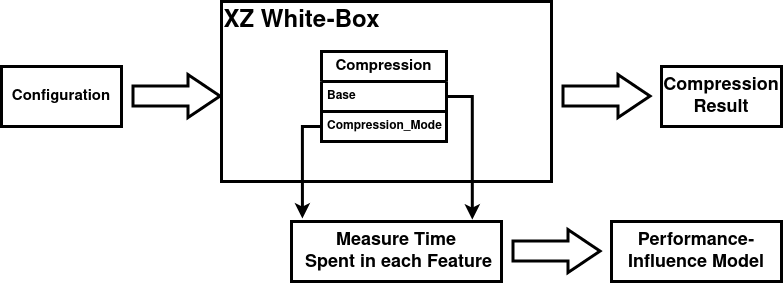
\includegraphics[scale=0.55]{gfx/whitebox_2.png}
    \caption{Process of using a black-box analysis to build a {\perfInfluenceModel} for \textit{XZ}.}
    \label{fig:WBxz}
\end{figure}

%Example of white-box pipeline
We now use a white-box analysis, to analyze the example system from \autoref{fig:xz}. 
In \autoref{fig:WBxz}, we have access to the source code of \textit{XZ}; 
our first step is to manually analyze the code and find the variables that implement configurability inside the system. 
In this example, we found the feature \textit{Base} and \textit{compression\_mode}. 
During compression, we use our white-box analysis to measure the time spent by \textit{XZ} in the different features. 
This example measures the time spent in $Base$ and $Compression\_Mode$. 
After the system finished the process, we collected all the measurements, which we then used to build a {\perfInfluenceModel} for this configuration.

%expain sections
In \autoref{analyzing-strats}, we explain the current state-of-the-art strategies used to analyze systems using white-box. 
Subsequently, in \autoref{VaRA} we introduce \textsc{VaRA}, the analyzing tool we use, and its underlying principles. 
In \autoref{trace-event}, we explain how to build the {\perfInfluenceModel} using the white-box data.

\subsection{Strategies}\label{analyzing-strats}
%Introducing 3 Strategies
When analyzing systems using a white-box approach, different strategies have been introduced. 
In this chapter, we explain three different strategies, \textsc{ConfigCrusher} and \textsc{Comprex}, 
both model configurability on a feature level, whereas Weber et al. introduce a strategy that models configurability on a method level.

%Config Crusher
Velez et al. introduced us to \textsc{ConfigCrusher} \cite{ConfigCrusher}, 
a white-box analysis that uses static data-flow analysis to see how features influence variables and the control flow of the system. 
In addition, ConfigCrusher leverages three insights about configurable systems from previous works, namely irrelevance, orthogonality, 
and low interaction degree. They use irrelevance to identify features relevant to the system's data flow, 
reducing the number of configurations required to analyze the system. They use orthogonality to identify features that do not interact with each other and, 
therefore, can be measured together. Since only a few features interact, 
\textsc{ConfigCrusher} focuses on the configurations with interacting features to reduce the number of configurations to be analyzed. 
From these findings, two techniques are developed, namely compression and composition. 
They use compression to reduce the number of configurations required to analyze the system by simultaneously analyzing regions that are independent of each other 
so that they can use a single configuration to analyze different features. 
Whereas composition takes advantage of the fact that {\perfInfluenceModel} can be built compositionally by building a performance-influcence model 
for each region separately and then assembling all local {\perfInfluenceModel} into one model for the entire system.
After using the data-flow analysis to generate a control flow graph and a statement influcence map, which maps statements to the configuration options 
that influence that statement.
Afterward, they use both the control flow graph and statement influcence map to instrument the regions in the system that correspond to features and execute
the instrumented system to track execution time of each feature. From these measurements, they build the {\perfInfluenceModel} for the system.

%Comprex
Velez et al. introduced \textsc{Comprex} \cite{Comprex}, an approach that builds on \textsc{ConfigCrusher} 
but uses an iterative dynamic taint analysis instead of static analysis to determine how and to what extent features affect the control flow of the given system.
By doing so, they identify which code regions are influenced by which configurations and, during execution measure the time spent in these regions to then build 
the {\perfInfluenceModel}.

%Method level
Compared to \textsc{ConfigCrusher} and \textsc{Comprex}, Weber et al. 
\cite{White-box-Profiling} uses a profiling approach to generate performance-influence models that analyze configurability on a method level. 
To achieve this, they first used \textsc{JProflier}, a coarse-grained profiler, 
to learn a performance-influence model for every method that has been learned successfully. To identify the hard-to-learn methods, 
they use filtering techniques and then \textsc{KIEKER}, a fine-grained profiler, to learn these methods. At the end, for each method, they
obtain a {\perfInfluenceModel} that shows how strong each feature influences the performance of that method.


\subsection{VaRA}\label{VaRA}
%what is vara
To analyze the system we are interested in, we use \textsc{VaRA}, a framework for analyzing configurable software systems that is built on \textsc{LLVM}.
In addition, we use the \textsc{VaRA Tool Suite}\footnote{Visited at 14.03.2022 \url{https://vara.readthedocs.io}}, which provides us with a framework that supports
us when analyzing configurable systems using \textsc{VaRA}.
    
%Why vara
The purpose of \textsc{VaRA} is to provide various analyses for systems where the user only needs to focus on the high-level conceptual information of the 
system, while \textsc{VaRA} handles the low-level-details. 
Since \textsc{VaRA} is built on top of \textsc{LLVM}, it is able to analyze systems written in languages that can be compiled by \textsc{LLVM}, such as C, C++ or Rust \cite{VaRA-Flo}.

\subsubsection{Feature Region}
%What a feature region is
To analyze configurable systems, \textsc{VaRA} identifies code regions associated with a feature or feature interaction; 
these regions are called \emph{feature region}. 
The first step for \textsc{VaRA} to be able to detect these regions is to find the feature variable that represents the features inside the code and mark them as
feature variables. 
A feature region is, therefore, a part of the code that is executed depending on the value of the feature variable. Whenever we detect a feature region,
we inject code into the system to measure the time spent in these regions.

\lstset{style=myStyle}
\begin{minipage}{\linewidth}
\begin{lstlisting}[caption={Feature region example},language=C++,label={alg:Vara_feature_regions},escapechar=|]
void encrypt() {
    bool Encryption; //Feature Variable | \label{line:encryption_feature_variable} |
    assign_feature(Encryption); //Assigns true if Encryption is selected
    
    if(Encryption) | \label{line:encryption} |
        foo();     | \label{line:foo} |
    else
        bar();      | \label{line:bar} |
}
\end{lstlisting}
\end{minipage}

%Feature region example
In \autoref{alg:Vara_feature_regions}, we can see the structure of the $Encryption$ feature region. 
The feature variable in \autorefLine{line:encryption_feature_variable} represents whether $Encryption$ is selected or deselected; depending on $Encryption$, 
either the $then$ or $else$ branch is executed. 
Together, these two branches form an $Encryption$ feature region.

\textsc{VaRA} uses different detection approaches to identify these feature regions, both of which use a \emph{taint analysis}.

%Explain taint analysis
\subsubsection{Taint Analysis}
Before explaining \textsc{VaRA} feature region detection, we explain the concept behind a taint analysis since both approaches build upon this analysis.

The common usage of a taint analysis is in cybersecurity, where we trace the data flow of data that originates from an outsider or an untrusted source; 
this input is labeled a \emph{tainted}. 
We then track how this tainted data is propagated through the system until it reaches a point where the data is again accessible to the outside. 
We call the access where the data is injected \emph{sources}, and the points where the data is extracted \emph{sinks} \cite{TaintAnalysis}.

%Expains vra taint analysis
\textsc{VaRA} uses taint analysis, too; however, in contrast to the common usage of a taint analysis, 
we are not interested in finding the sinks where data is leaked to the outside. However, instead, we are interested whenever instructions access our feature. 
For the taint analysis, \textsc{VaRA} uses feature variables as sources and instruction as sinks. Whenever an instruction accesses a feature variable, 
this instruction is tainted by that feature \cite{VaRA-Janik}.

\textsc{VaRA} uses the taint analysis in both approaches, the \emph{if approach} and \emph{dominator approach}, to detect feature regions.

%Explain IF approach
\paragraph{If Approach}
We call the first approach the \emph{if approach}. Here, whenever a feature variable that was declared as a source is accessed in the condition of an if statement, 
then the \emph{then} case and the \emph{else} case are marked as a feature region \cite{VaRA-Tom}.

In \autoref{alg:Vara_feature_regions} in \autorefLine{line:encryption} an if condition access the feature variable \emph{Encryption}, 
here the if approach would mark \autorefLine{line:foo} and \autorefLine{line:bar} as a feature region of \emph{Encryption}.

%Expain Dominator approach
\paragraph{Dominator Approach}
We call the second approach the \emph{Dominator Approach}, in here, \textsc{VaRA} uses domination relationships to identify feature regions.

To do this, \textsc{VaRA} works with basic blocks of the control flow graph, whereas a basic block is an instruction sequence that contains an entry label, 
which is the entry point for this code, and a terminator at the end, which determine the control flow of the block. 
An example of a terminator is an if condition that uses a feature variable.

To discover these domination relationships, \textsc{VaRA} checks out which basic block dominates other basic blocks with dependent terminator instructions. 
A basic block $BB_1$ dominates a different basic block $BB_2$ when the terminator of $BB_1$ decides if $BB_2$ is executed. 
Now instructions in $BB_2$ would depend on the terminator instruction of $BB_1$. 
The feature for the feature region of $BB_2$ is the feature that corresponds to the feature variable used by the terminator of $BB_2$ \cite{VaRA-Tom}.


\subsubsection{Locating feature variables}
\textsc{VaRA} is not able to automatically detect which variables represent features. 
Therefore, we provide \textsc{VaRA} with a feature model as a \textsc{XML} file containing every feature's location inside the code.

\begin{minipage}{\linewidth}
\begin{lstlisting}[caption={Feature model of \autoref{alg:Vara_feature_regions} in XML},language=XML,label={alg:Encrypton_feature_model_xml},escapechar=|]
<?xml version="1.0" encoding="UTF-8"?>
<!DOCTYPE vm SYSTEM "vm.dtd">
<vm name="SingleLocalSingle" root="root">
    <binaryOptions>                               | \label{XML:binary_option} |
        <configurationOption>                     | \label{XML:config_option} |
        <name>Encryption</name>                   | \label{XML:name} |
        <parent></parent>
        <optional>True</optional>
        <locations>                               | \label{XML:location} |
            <sourceRange category="necessary">    | \label{XML:source_range} |
                <path>src/my_encryption.c</path>      | \label{XML:file_path} |
                <start>                               | \label{XML:start_variable} |
                    <line>2</line>
                    <column>10</column>
                </start>
                <end>                                 | \label{XML:end_variable} |
                    <line>2</line>
                    <column>19</column>
                </end>
                </sourceRange>
        </locations>
        </configurationOption>
    </binaryOptions>
    <numericOptions></numericOptions>             | \label{XML:numeric_option} |
    <booleanConstraints/>
</vm>
\end{lstlisting}
\end{minipage}

%XML Lplained
As an example \autoref{alg:Encrypton_feature_model_xml} encodes \autoref{alg:Vara_feature_regions} as a feature model. 
Inside the \textsc{XML} we differentiate between two kinds of feature, \emph{<binaryOptions>} in \autorefLine{XML:binary_option} and \emph{<numericOptions>} in 
\autorefLine{XML:numeric_option}, we declare each feature as a child of either those two tags. We encapsule every feature we want to 
track by using the \emph{<configurationOption>} tag in \autorefLine{XML:config_option}, inside we can define the \emph{<name>} of the feature, in \autorefLine{XML:name}
its parent, and if the feature is optional, but most importantly in \autorefLine{XML:location} we define the \emph{<location>} to specify
where the feature variable is defined inside the code.
The location tag contains, at least one \emph{<sourceRange>} tag, in which we specify the feature variable that is associated with the feature, 
however a location can contain multiple source ranges, whereas the feature is implemented by multiple feature variables.
Each \emph{<sourceRange>} tag contains a \emph{<path>} tag that specifies the location of the file containing the feature variable.
After specifying the path, we need even further to specify the location of the feature variable inside the file. 
For this, we see in \autorefLine{XML:start_variable} the \emph{<start>} tag and in \autorefLine{XML:end_variable} the \emph{<end>} tag, 
inside both, we specify the \emph{<line>} and \emph{<column>} for where the feature variable starts end ends. 

%Explained on example
For \autoref{alg:Vara_feature_regions}, we would specify that the feature variable
$Encryption$ is in \autorefLine{line:encryption_feature_variable} and begins in \emph{column 10} and ends in \emph{column 19}.

After identifying all the feature regions of each feature, we run \textit{VaRA}, together with the feature model, to locate all feature regions \cite{VaRA-Flo}.

\subsubsection{VaRA Tool Suite}
%Explain Vara Tool Suite
We use \textsc{VaRA} in combination with the \textsc{VaRA Tool Suite}, a framework written in python that assists us 
when analyzing configurable software systems using \textsc{VaRA} by specifying an \emph{experiment} to analyze a particular \emph{project}. 
The result our analysis produces is written into a \emph{report}. We emphasize that both experiments and projects are independent, 
allowing us to use different experiments to analyze a project in different ways.
To start the analysis, we use the command-line tool \emph{vara-run}, which specifies which experiments we want to run for which project.

\paragraph{Project}
A \emph{project} inside the \textsc{VaRA Tool Suite} specifies the configurable software system we want to analyze. 
Here we define how we build the system or which version of the system we want to study.

In our example of \autoref{fig:WBxz}, the project would be \textsc{XZ} and would specify which version of \textsc{XZ} we want to analyze and how the binary is build.

\paragraph{Experiment}
Inside \textsc{VaRA Tool Suite} an \emph{experiment} specifies how we want to analyze a software project. This allows us to make the analysis
easy to reproduce and repeat.

In \autoref{fig:WBxz} we want to analyze \textsc{XZ}, in the experiment we specify that we want to use \textsc{VaRA} and the different steps we want to execute,
like which report we want to use.

\paragraph{Report}
\textsc{VaRA} Tool Suite offers us a variety of \emph{reports} which are used to store different data, which we generate during the analysis.

For \autoref{fig:WBxz} we use the trace event format report which we explain in \autoref{trace-event}


\subsection{Trace Event Format}\label{trace-event}
%Introduce TEF report and purpose
When we use \textsc{VaRA} the code of the configurable software system gets instrumented to measure the time spent inside each feature region. 
During the execution of the whole system, we enter various feature regions multiple times.
We collect all these measurements
in a trace event format (TEF) \footnote{Visited at 15.03.2022 \\ \url{https://docs.google.com/document/d/1CvAClvFfyA5R-PhYUmn5OOQtYMH4h6I0nSsKchNAySU}} report.

Every time we enter or leave a feature region, a trace event is triggered that contains the following information:\\

\begin{minipage}{\linewidth}
\begin{lstlisting}[caption={Trace event},captionpos=b,language=json,firstnumber=1,label={event}]
"name": "Base",
"cat": "Feature",
"ph": "B",
"ts": 0,
"pid": 726119,
"tid": 726119,
"args": {
    "ID": 0
}
\end{lstlisting}
\end{minipage}
%Expain all the keys meaning
In \autoref{event}, we see how a trace event is structured. Each trace event contains a $name$ that refers to the names of the features that affect this
region, $ph$ represents the event type, while $B$ signals the beginning and $E$ the end of an event.
All events contain a timestamp $ts$ that refers to the time in milliseconds when the event began or ended.
$Args$ contain an $ID$ that refers to each event, so the event that initiates the beginning $E$ of a region has the same $ID$ as the event that signals when
we leave the region with $E$.

%explain feature interaction time spent
When a trace event for a feature region begins before a trace event for a different feature ends, we say these features interact. 
As an example, if we have two features, \emph{foo} and \emph{bar}, where the trace event of \emph{foo} starts at \emph{0} and ends at \emph{4} seconds 
and the trace event of \emph{bar} starts at \emph{1} and ends at \emph{3} seconds. We spent \emph{2} seconds in feature \emph{foo}, 
from \emph{0 to 1} and \emph{3 to 4}, 
but since we did not leave the feature region \emph{foo} before entering \emph{bar} we have an interaction between these features. 
Therefore, we spent \emph{2} seconds inside the feature interaction \emph{(foo, bar)} instead of the feature \emph{bar}.

%Expain order of interaction is irrelevant
Since we are only interested in which features interact, we ignore the order in which the interaction happens, which means the previous
interaction of \emph{(foo, bar)} is the same as \emph{(bar, foo)}. This also makes sense in the context of {\perfInfluenceModel} since we defined
the interaction of features as a product, where the time spent in that feature interaction is added if all features of that interaction are selected,
in this case, $2 \cdot c(foo) \cdot c(bar)$. Since the product is commutative, we also ignore the order in which the features interact inside the \perfInfluenceModel.

%Expain nesting
When we have nested trace events of the same feature, we do not add a feature interaction between the same features, 
due to the reason that inside the {\perfInfluenceModel} the feature interaction $2 \cdot c(foo) \cdot c(foo)$ is the same as $2 \cdot c(foo)$.

After the system finishes its execution, we have to transform the TEF report into a {\perfInfluenceModel} by aggregating all events. 
To do so, we sum up all the time spent in each region and attribute this time to the feature that influenced that region. 

We calculate the time spent on each feature as follows:

\mycomment{\begin{algorithm}
    \caption{Time spent in each feature \label{alg:performanceExample}}
    \textbf{Input:} feature_trace_event, a list containing features and
    \begin{algorithmic}[1]
    \text
    \State $\textit{features} \gets \textit{list}$\label{alg:code_insertion}

    \end{algorithmic}
    \end{algorithm}
}

\begin{align}
    time(feature) &= \textit{ }\textit{ }\textit{ } \sum_{event \in feature} \left( \sum_{(ts_E, ts_B) \in event} ts_E - ts_B \right) \label{math:time}\\ \nonumber \\
    feature\_coefficients &= \sum_{feature \in TEFReport}time(feature) \label{math:coefficients}
\end{align}

In \autoref{math:time}, we calculate the time spent for the given feature. 
For this equation, we define that a \textit{feature} is a list of \textit{events}, 
whereas each event is a pair of trace events representing when the feature region is entered and when it is left. 
To calculate the time spent in the region, we compute $ts_E - ts_B$.

\autoref{math:coefficients} is a sequence of the total time spent in each feature or feature interaction we measured in the \textit{TEF Report}. 
Now that we obtained all the coefficients that represent the influence of each feature and feature interaction, we use them to build the \perfInfluenceModel.
